\documentclass[a4paper, dutch, abstract=true]{scrartcl}
\usepackage[utf8]{inputenc}
\usepackage[dutch]{babel}
\usepackage{graphicx}
\graphicspath{{./afbeeldingen/}}
\usepackage[automark]{scrlayer-scrpage}
\usepackage[style=ieee]{biblatex}
\addbibresource{raspberry-pi.bib}
\title{Vergelijking het Raspberry Pi- en Arduinoplatform}
\subtitle{Papergroep 34}
\subject{INFONW Paper}
\author{
    Wilmar Duvekot 6523617 \and Luuk Berkers 6793592 \and Jacob-Jan Mosselman
    6675522 \and Kenneth Man 6007767 \and Herman Horneman 6897630
}
\date{28 oktober 2019}
\addtokomafont{pagehead}{\upshape}

\begin{document}
\maketitle

\begin{abstract}
    Dit onderzoek probeert een antwoord te geven op de vraag of een Arduino of een Raspberry Pi een
    betere mini-computer is.
    Het onderzoek geeft daarop een antwoord en ook op de vraag wat de verschillen precies zijn.
    De Arduino is een mini-computer die vooral handig kan zijn bij het automatiseren van processen,
    en de Raspberry Pi is een iets uitgebreidere computer met wat meer aansluitingen beschikbaar.
    Het grootste verschil is dat de Raspberry Pi een grotere processor heeft dan de Arduino.
    Hieruit wordt geconcludeerd dat de Raspberry Pi het beste gebruikt kan worden voor grote
    opdrachten en dat de Arduino geschikt is voor kleinere, simpele opdrachten.
\end{abstract}

\tableofcontents

\section{Inleiding}
In de laatste decennia heeft technologie een enorme ontwikkeling doorgemaakt.
Zo zijn de telefoons uitgevonden en zijn deze steeds kleiner, sneller en beter geworden.
Televisie heeft kleur gekregen en er zijn steeds meer zenders te zien.
Ook heeft de computer een enorme ontwikkeling doorgemaakt.
De computers van vroeger konden klaslokalen vullen, maar tegenwoordig kunnen ze in een rugzak
meegenomen worden.
De laptop wordt steeds kleiner, steeds sneller en gaat ook steeds beter presteren.
De technologie gaat tegenwoordig zelfs zo ver, dat een fotolijstje digitaal gemaakt kan worden,
zodat mensen foto's naar het lijstje kunnen sturen en dat het lijstje die foto's dan laat zien, een
voorbeeld daarvan is de Claudia digitale fotolijst \cite{innovu2019fotolijst}.

De technologie wordt steeds kleiner en beter dus, dat is ook te zien aan de mini-computers.
De Raspberry Pi \cite{raspberry2019raspberry} en de Arduino \cite{arduino2019arduino} zijn ongeveer
even groot als een telefoon en ze kunnen veel.
Het principe is hetzelfde als een laptop of computer
De computers kunnen worden geprogrammeerd, en ze kunnen in principe alles doen, zolang het
geprogrammeerd wordt.
De Arduino en Raspberry Pi zullen in dit onderzoek verder uitgelegd worden.

Dit onderzoek zal gaan over de verschillen tussen de Arduino en Raspberry Pi, zodat duidelijk wordt
wat met de mini-computers gedaan kan worden en wat het nut kan zijn in de samenleving.
De onderzoeksvraag luidt: Wat zijn de verschillen tussen Raspberry Pi en Arduino en welke is beter?
Op deze vraag zal een antwoord gevonden worden in dit paper.
Dit paper zal beginnen met informatie over de Arduino, de architectuur, hardware, software en
toepassingen.
Vervolgens zal er worden verteld over de Raspberry Pi, architectuur, hardware, software en
toepassingen.
Daarna zullen verschillen en overeenkomsten besproken worden.
Vervolgens volgt de conclusie en de appendix.

\section{Arduino}
Dit paper zal beginnen met te vertellen hoe een Arduino in elkaar zit.
Dit zal gebeuren aan de hand van de architectuur en de hardware van de Arduino.
Vervolgens wordt er gekeken naar de software van de Arduino en er wordt als laatst gekeken naar de
toepassingen en mogelijkheden.
\\

Er is nu bekend wat de Arduino kan en hoe deze werkt
Om de onderzoeksvraag volledig te kunnen beantwoorden is het goed om zowel over de Arduino als over
de Raspberry Pi informatie te hebben.
Het volgende stuk in dit paper zal gaan over de Raspberry Pi en hoe deze werkt.

\section{Raspberry Pi}
Zoals in het vorige stuk genoemd, is het nodig om de mogelijkheden van de Raspberry Pi te
begrijpen om de onderzoeksvraag goed te beantwoorden.
Dit zal gaan op dezelfde manier als de Arduino ook is uitgelegd.
Eerst zal worden gekeken naar de architectuur en hardware.
Vervolgens naar de software van een Raspberry Pi en op het eind zullen toepassingen en mogelijkheden
besproken worden.

\subsection{Architectuur \& Hardware}
De Raspberry Pi is een volwaardige computer met een compact formaat.
Hij bevat dezelfde componenten die een volledige desktop-pc ook bevat, met als voordeel dat hij in
een broekzak past.
Bijkomend nadeel is wel dat men een aparte monitor, muis en toetsenbord moet aanschaffen als men de
Raspberry Pi als traditionele desktop computer wilt gebruiken.

In tegenstelling tot traditionele desktop pc's en laptops van de laatste 10 jaar is de Raspberry Pi
niet voorzien van een x86 processor.
De Raspberry Pi is voorzien van een ARM processor \cite{jain2014raspberry}.
Er bestaan op het moment van schrijven verschillen versies.
De Raspberry Pi 1 en Zero hebben een 32-bits architectuur, terwijl de Raspberry Pi's 2, 3 en 4 een
64-bits architectuur hebben.
Verder is de architectuur min of meer hetzelfde.
Alle Raspberry Pi's draaien op basis van een ARM processor.

Omdat er verschillende versies bestaan van de Raspberry Pi, wordt in dit paper de nadruk gelegd op
de Raspberry Pi 4.
Deze heeft een kloksnelheid van 1.5 GHz en een RAM van 1, 2 of 4 GB.
Afhankelijk van het Raspberry Pi 4 model dat men gekocht heeft, zal het RAM geheugen verschillend
zijn.
Kloksnelheid is wel voor alle modellen van de Raspberry Pi 4 hetzelfde.
Verder heeft hij in totaal vier USB poorten.
Namelijk twee USB 2.0 en 2 USB 3.0 poorten.
Ook heeft de Raspberry Pi 4 een Ethernet aansluiting waarmee een internetverbinding mogelijk is,
maar ook een directe verbinding met een andere computer \cite{maksimovic2014raspberry}.
Voor een internetverbinding beschikt de Raspberry Pi ook over wifi functionaliteit.

\subsection{Software}
\begin{figure}[h]
    \centering
    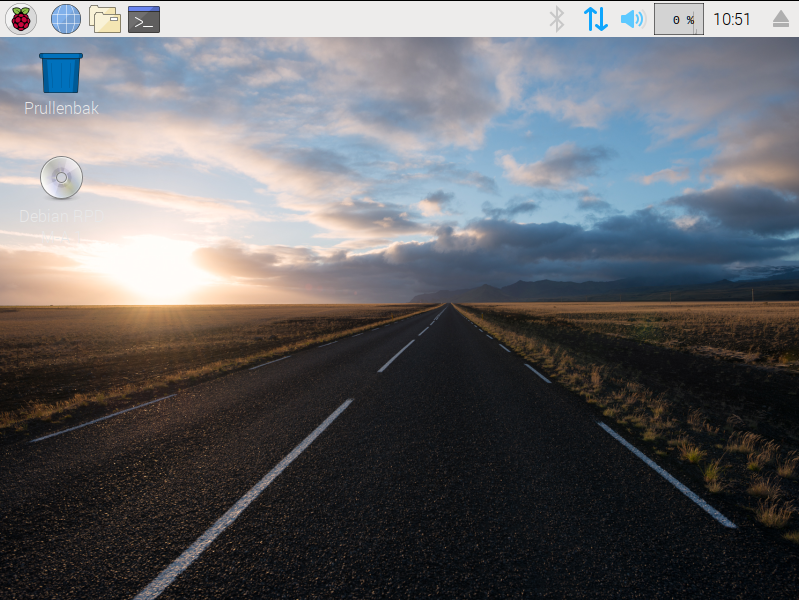
\includegraphics[scale=0.5]{raspbian.png}
    \caption{Raspbian desktopomgeving}
    \label{fig:raspbian}
\end{figure}
\begin{figure}[h]
    \centering
    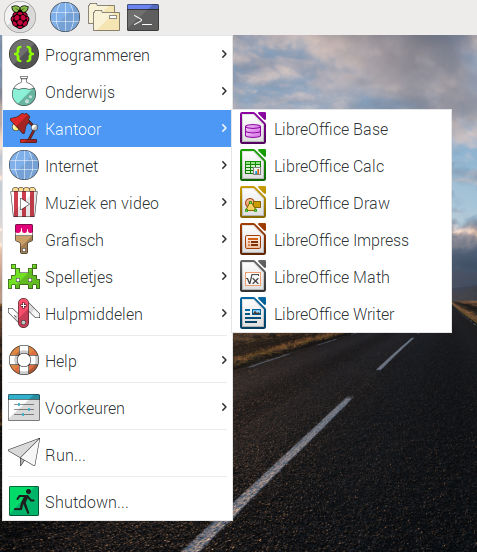
\includegraphics[scale=0.5]{raspbian-libreoffice.png}
    \caption{Raspbian heeft LibreOffice als kantoorsoftwarepakket}
    \label{fig:raspbian-libreoffice}
\end{figure}
Afhankelijk van het besturingssysteem dat draait op de Raspberry Pi 4, zijn een aantal software al
ge{\"i}nstalleerd.
Men kan er ook voor kiezen om een versie te installeren zonder deze voorge{\"i}nstalleerde software.
De Raspberry Pi Foundation ontwikkelt zelf een besturingssysteem voor de Raspberry Pi.
Dit besturingssysteem heet Raspbian en is gebaseerd op Debian.
In figuur \ref{fig:raspbian} is het bureaublad weergegeven van de versie van Raspbian met een
desktopomgeving.

Er is in dit paper ervoor gekozen om Raspbian te installeren met voorge{\"i}nstalleerde software.
Als men met de muis klikt op de framboos in de linkerbovenhoek, dan zal men verschillende software
aantreffen zoals te zien is in figuur \ref{fig:raspbian-libreoffice}.
Zo is bijvoorbeeld te zien dat Raspbian beschikt over LibreOffice.
Dit is tekstverwerkingssoftware vergelijkbaar met Microsoft Office.

Naast tekstverwerkingssoftware is er ook een browser.
Standaard in Raspbian is de Chromium Web Browser.
Ook bevat Raspbian een Terminal applicatie waarin men via commando's opdrachten kan uitvoeren.

\subsection{Mogelijkheden \& Toepassingen}
\begin{figure}[h]
    \centering
    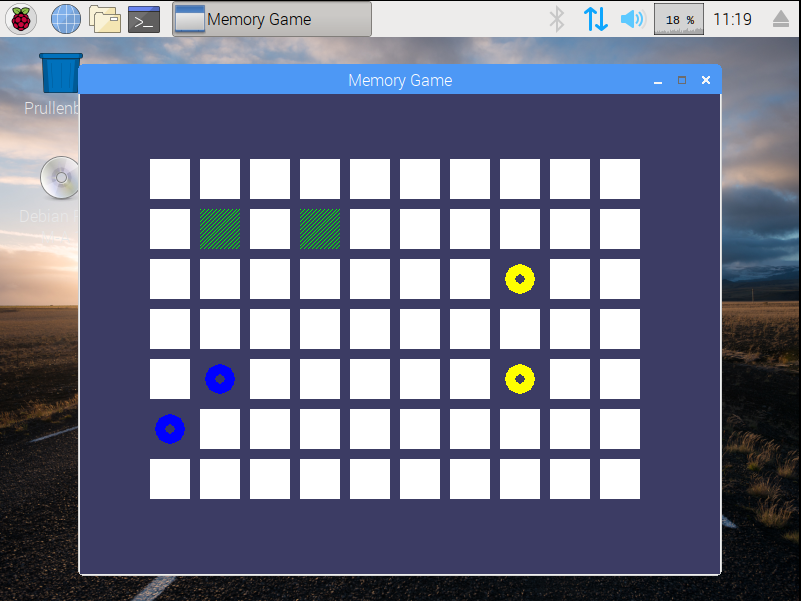
\includegraphics[scale=0.25]{raspbian-memory.png}
    \caption{Memory spel in Raspbian}
    \label{fig:raspbian-memory}
\end{figure}
Zoals al eerder gezegd is Raspberry Pi 4 een volledige computer.
Het enige verschil is dat hij in een formaat van een creditcard is.
Hij is dus erg compact en makkelijk te verwerken in allerlei projecten.
Met een Raspberry Pi 4 is het dus gewoon mogelijk om documenten te typen en om websites te bezoeken.

Echter heeft Raspberry Pi 4 ook flink een aantal nadelen.
Vanwege het ontbreken van een monitor, muis en toetsenbord, zal men deze apart moeten aanschaffen
als men de Raspberry Pi als desktop-computer wilt gebruiken.
Daarnaast is de kloksnelheid heel erg laag, namelijk 1.5 GHz.
Ook is het maximale beschikbare RAM geheugen heel erg weinig.

Ondanks deze beperkingen, zijn de mogelijkheden en toepassingen niet onaardig.
De simpele basistaken zoals tekstverwerking, internet en zeer lichte spelletjes spelen zijn gewoon
mogelijk.
Ter illustratie is in figuur \ref{fig:raspbian-memory} een simpele Memory spel te zien dat te spelen
is in Raspbian.

\section{Overeenkomsten en Verschillen}
In de vorige stukken zijn de eigenschappen, mogelijkheden en toepassingen van het Raspberry Pi- en
Arduino platform besproken.
In dit stuk zullen we de platformen vergelijken en de verschillen en overeenkomsten bespreken.
Deze bevindingen kunnen we dan vervolgens in de conclusie gebruiken om onze onderzoeksvraag te
beantwoorden.

\subsection{Architectuur \& Hardware}
Beide platformen zijn bedoeld voor gebruik in projecten waarin een computer nodig is, maar niet te
veel computer, dit is ook zichtbaar in het ontwerp van de hardware.
De afmeting van de Raspberry Pi 4 \cite{raspberry2019brief} zijn vergelijkbaar met verschillende
Arduino modellen, zoals de Arduino MEGA 2560 \cite{arduino2019mega} en de Arduino Uno
\cite{arduino2019uno}.
Daarnaast zijn er binnen beide platformen kleinere versies verkrijgbaar zoals de Raspberry Pi Zero
\cite{raspberry2019buy} en de Arduino Nano \cite{arduino2019products}.
Dit laat een belangrijke overeenkomst tussen de twee platformen zien, namelijk de focus op
compactheid.
Dit zorgt er voor dat de apparaten verwerkt kunnen worden in allerlei projecten, maar ook maakt het
de platformen toegankelijk voor niet-professionele toepassingen.
Denk aan hobbyisten die geen computer willen toewijden aan 1 taak, laat staan een serverkast gaan
opstellen.

De I/O van de Raspberry Pi, die bestaat uit USB, Micro HDMI en Ethernet \cite{raspberry20194bspecs},
is niet vergelijkbaar met bijvoorbeeld de Arduino Uno of MEGA 2560.
Bij Arduino's is de I/O vooral gebaseerd op digitale input/output pins
\cite{arduino2019mega,arduino2019uno}.
De I/O van de Raspberry Pi is wel vergelijkbaar met die van de Arduino Y{\'U}N, deze heeft als een
van de weinige Arduino's USB en Ethernet.
Deze Arduino is dan ook ontworpen om gebruikt te worden wanneer een internetverbinding nodig is
\cite{arduino2019yun}.
Dit laat een verschil zien in de doeleinden waarvoor de computers binnen de platformen ontworpen
zijn.
De Arduino is nuttig wanneer I/O op laag niveau nodig is, met volledige controle over elke bit van
in- en uitvoer.
De Raspberry Pi heeft de mogelijkheid om op een netwerk aangesloten te worden, en ook kan er
standaard USB-randapparatuur op aangesloten worden, dit maakt de Raspberry Pi nuttig voor projecten
waarbij I/O op hoger niveau nodig is.
Het verschil is ook niet vreemd wanneer rekening gehouden wordt met het feit dat de Raspberry Pi een
OS heeft om deze I/O aan te sturen, terwijl de Arduino dit niet heeft.
\\

% \section{Software}
% Zoals eerder gezegd zijn beide platformen nuttig voor gebruik in projecten, zowel voor hobbyisten
% als professionele toepassingen.
% Beide platformen zijn dan ook heel makkelijk te programmeren en nuttig als middel om te leren
% programmeren \cite{raspberry2015what,jamieson2011arduino,rubio2013using}.

De overeenkomsten en verschillen zijn nu benoemd en uitgelegd, deze zullen worden gebruikt in het
volgende hoofdstuk, dat zal de conclusie zijn.

\printbibliography
\end{document}
